
\section{Results}
\subsection{Segmentation}


\begin{figure}[h]
	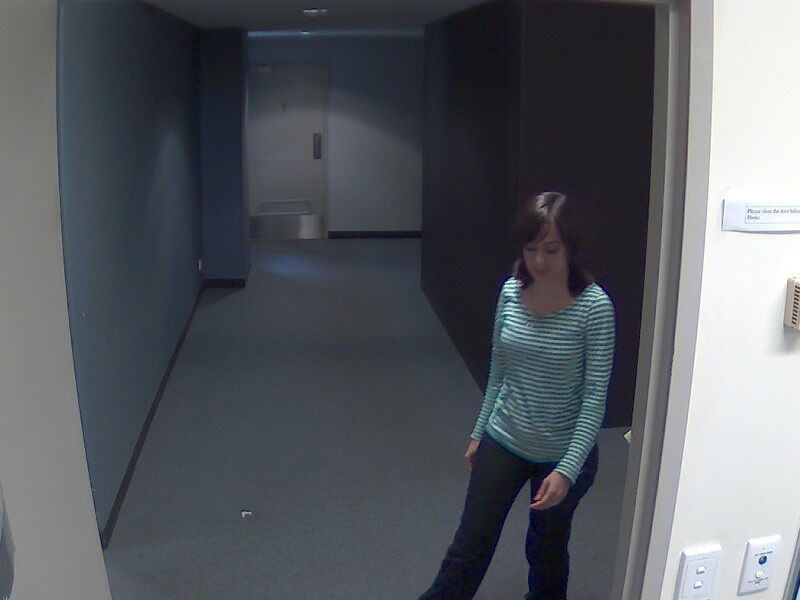
\includegraphics[width=12cm]{P1E_S1_ori}
	\caption{original image from P1ES1}
	\label{fig:original image from P1LS1}
\end{figure}

\begin{figure}[h]
	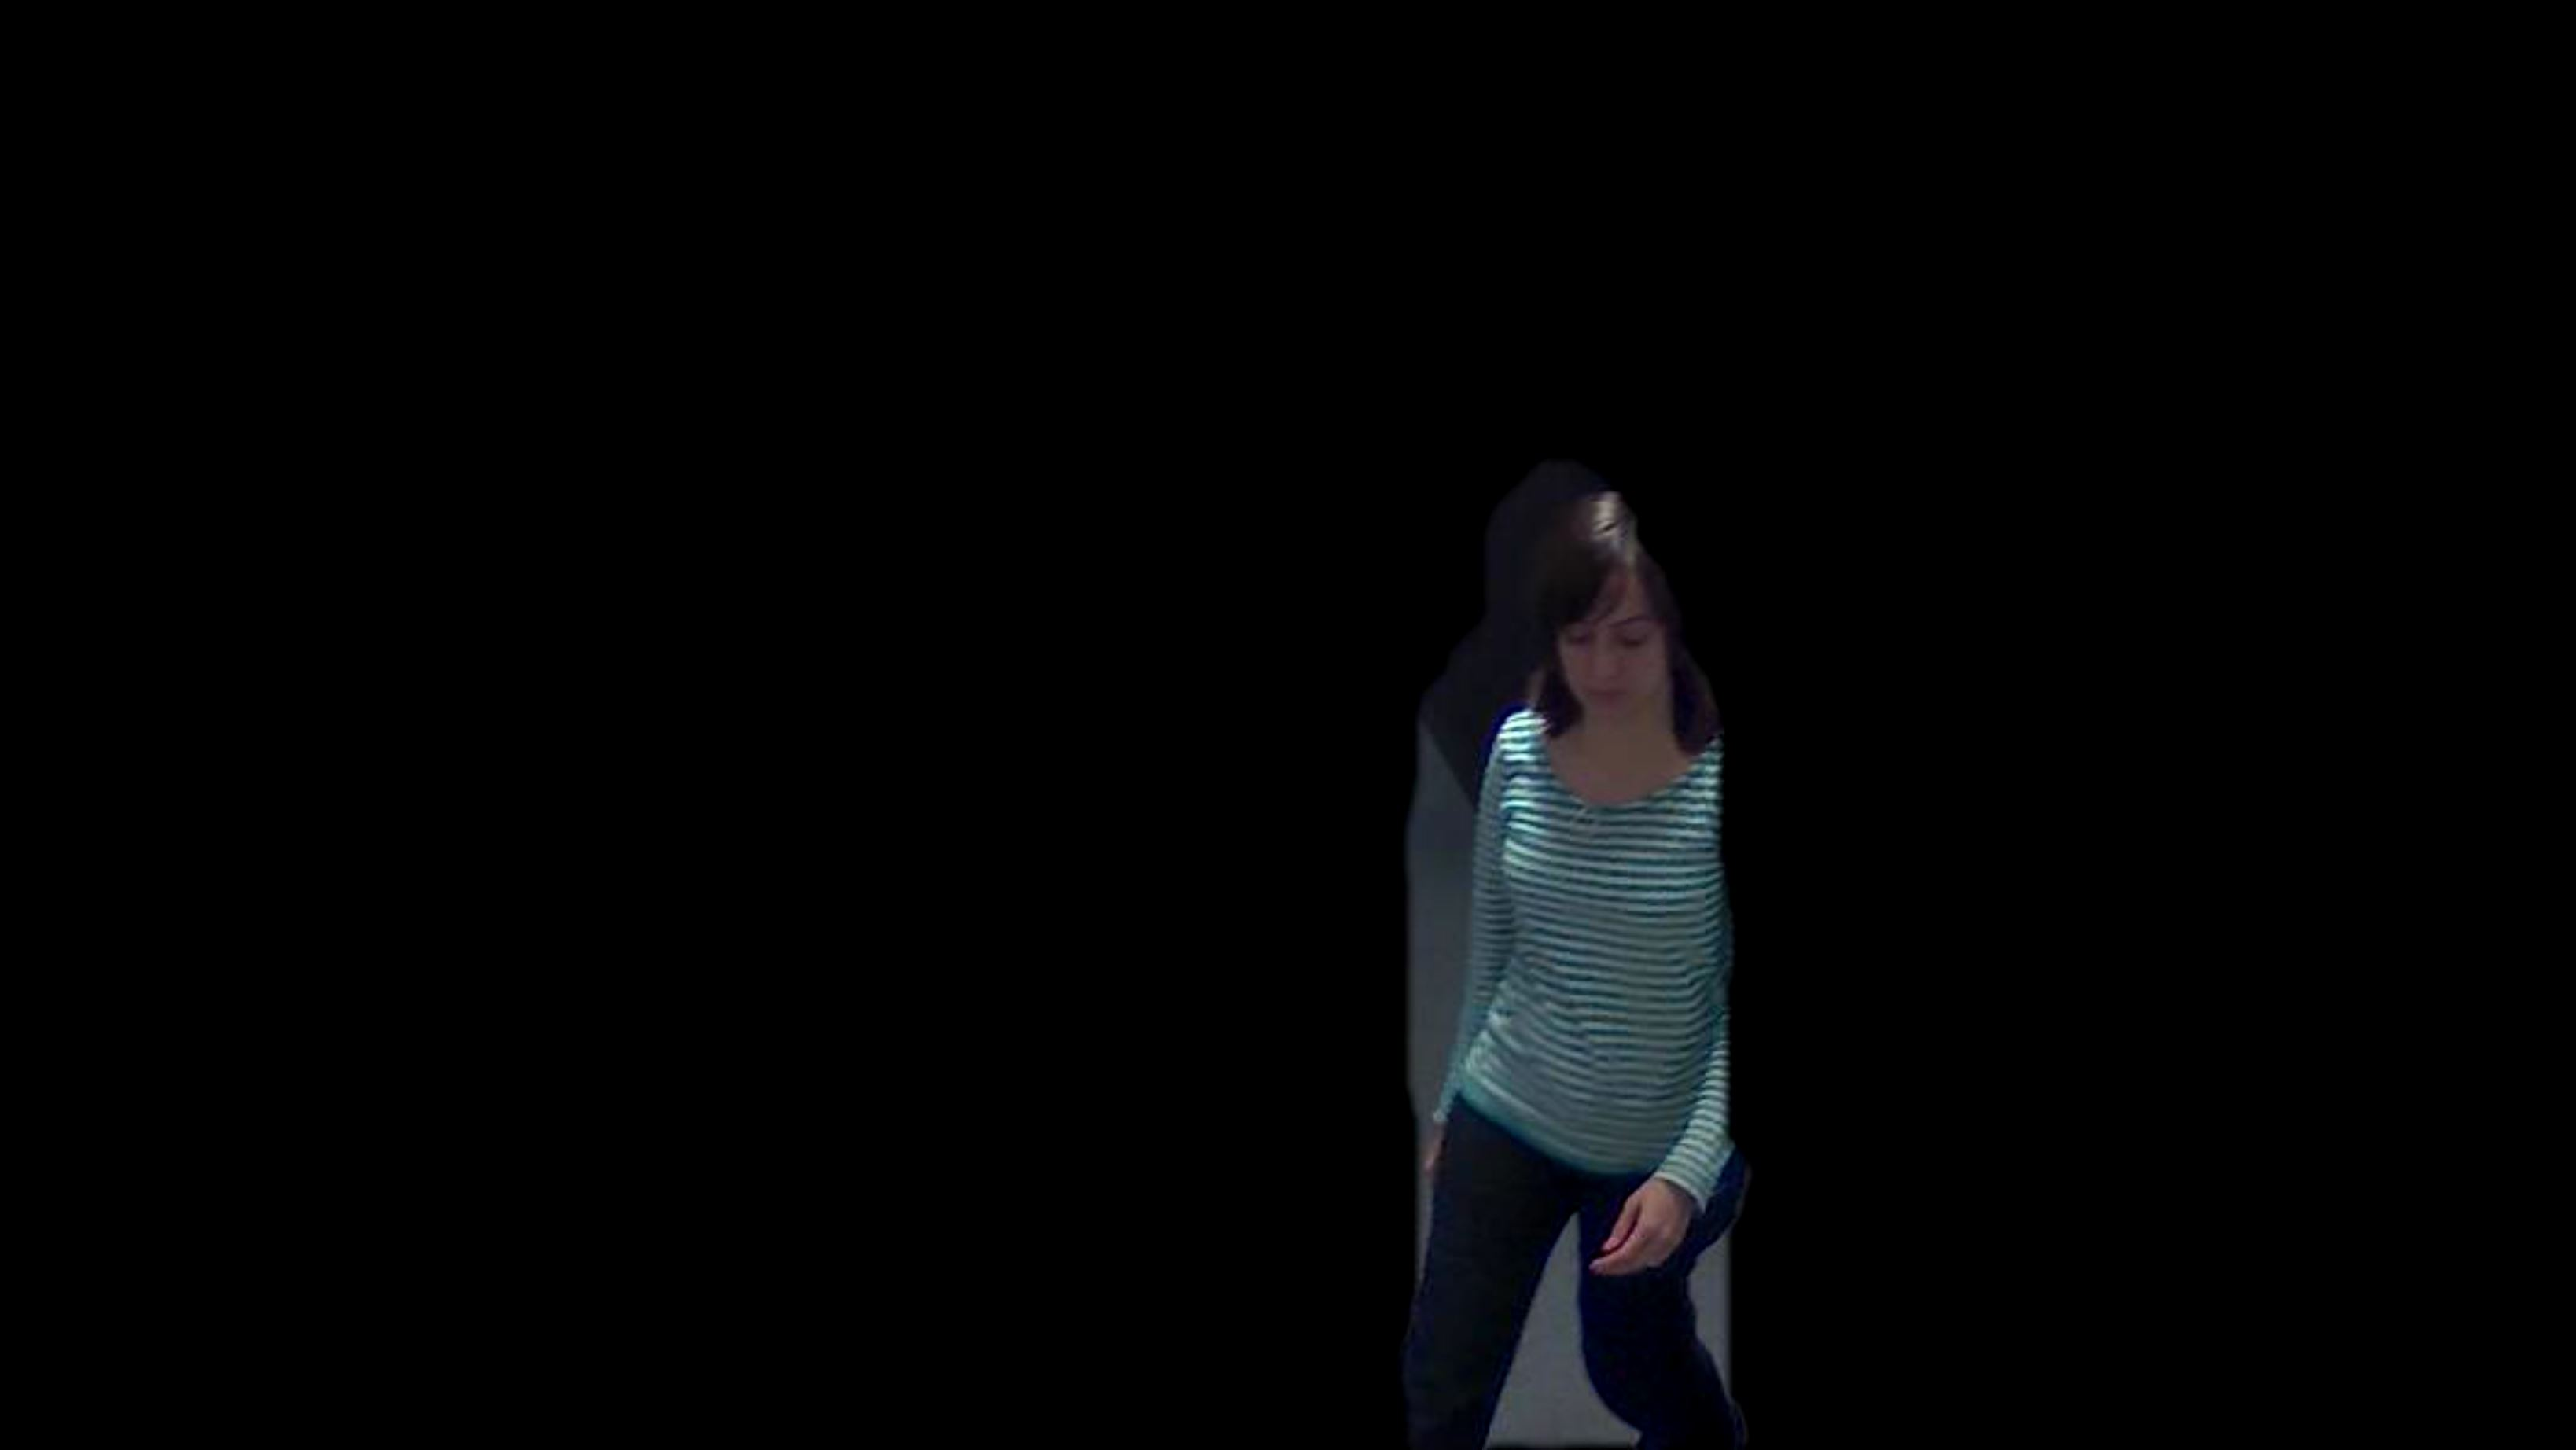
\includegraphics[width=12cm]{P1E_S1}
	\caption{rendered image from P1ES1}
	\label{fig:rendered image from P1LS1}
\end{figure}

\begin{figure}[h]
	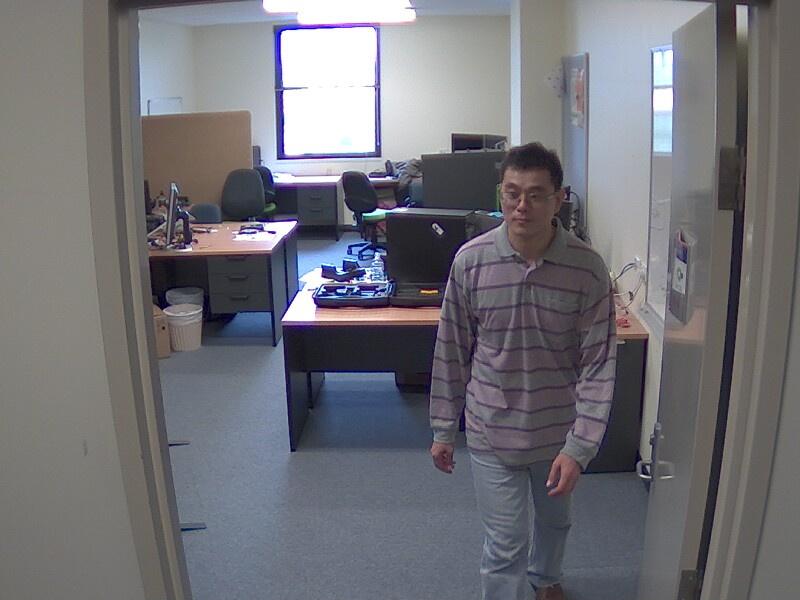
\includegraphics[width=12cm]{P1L_S3_ori}
	\caption{original image from P1LS3}
	\label{fig:original image from P1LS3}
\end{figure}

\begin{figure}[h]
	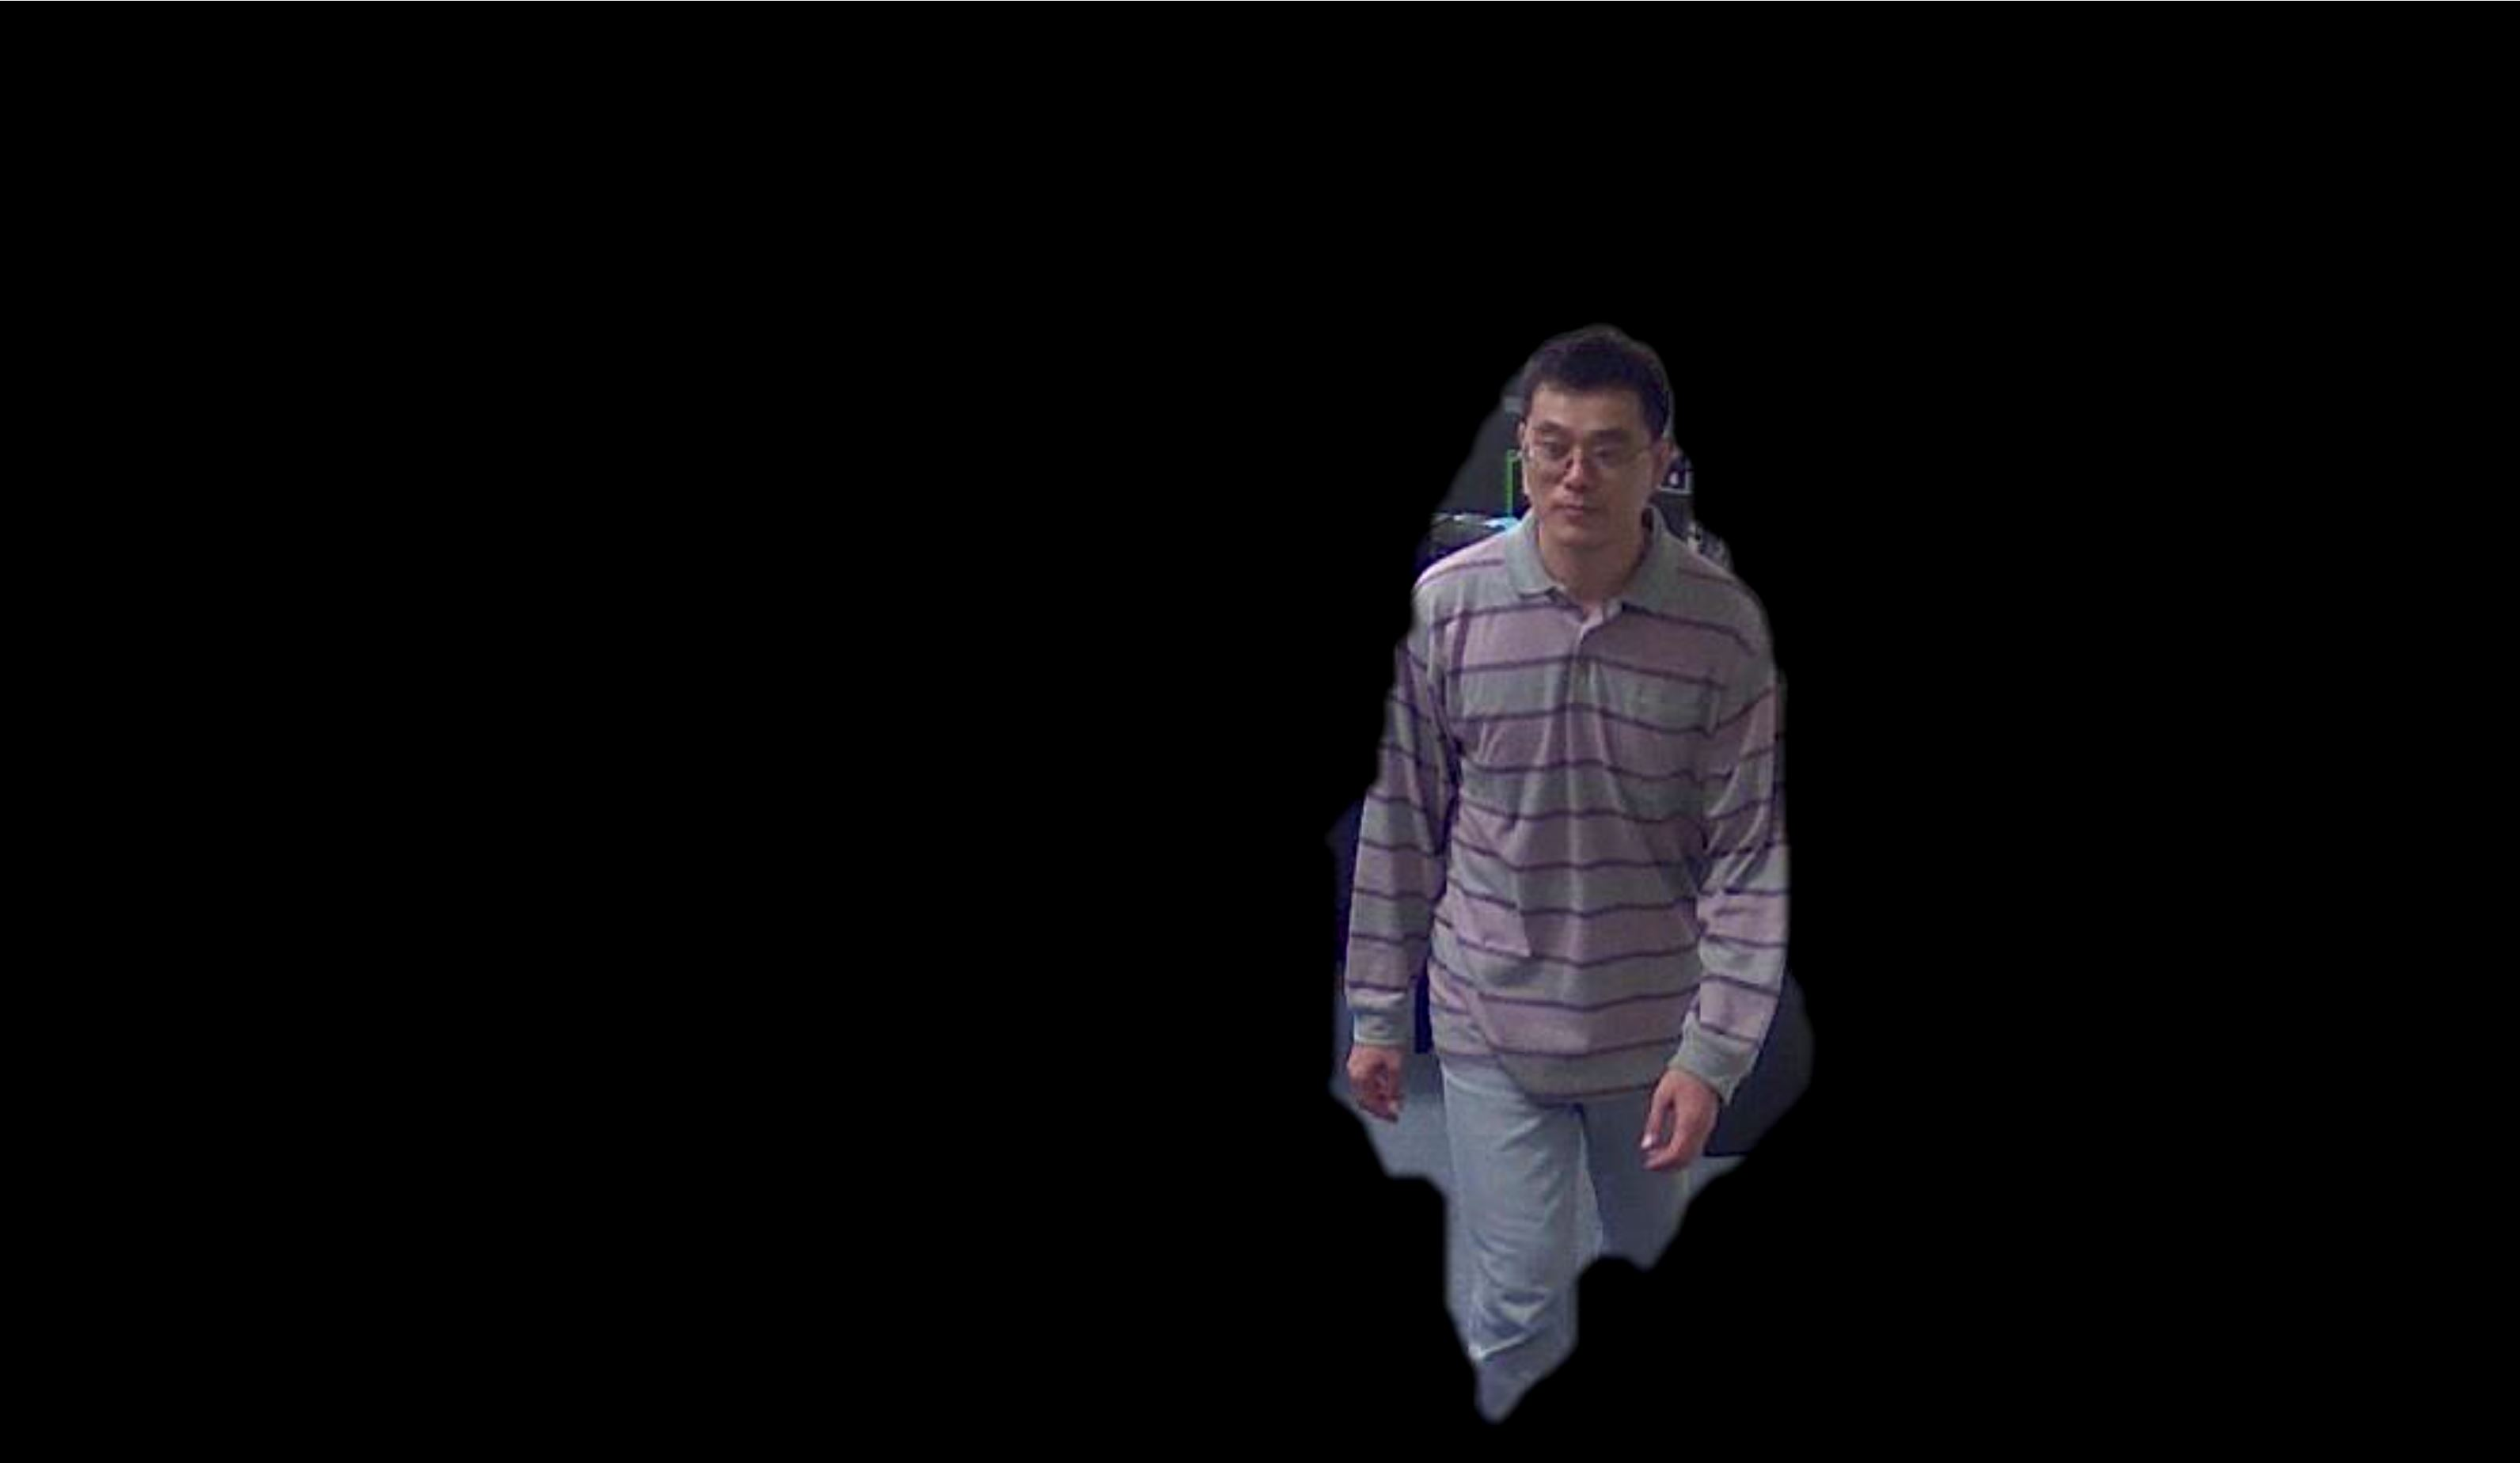
\includegraphics[width=12cm]{P1L_S3}
	\caption{rendered image from P1LS3}
	\label{fig:rendered image from P1LS3}
	
\end{figure}

\begin{figure}[h]
	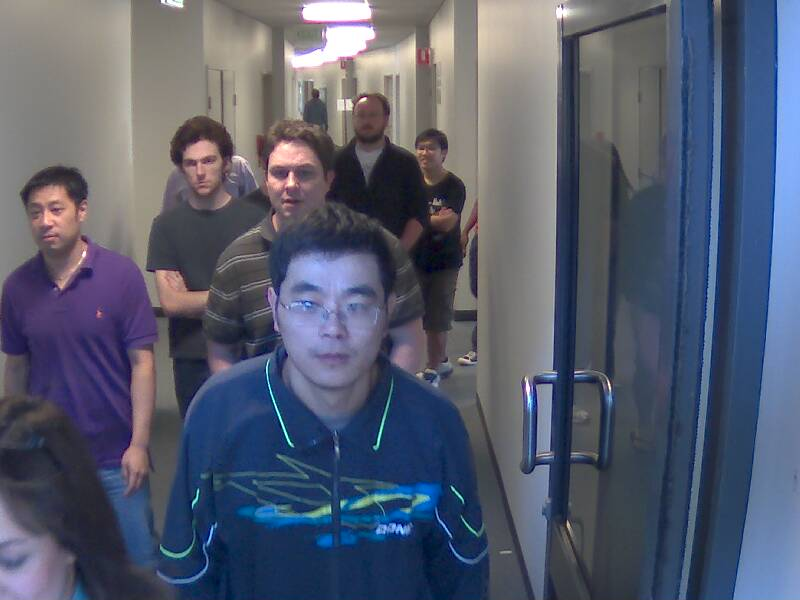
\includegraphics[width=12cm]{P2L_S5_ori}
	\caption{original image from P2LS5}
	\label{fig:original image from P2LS5}
\end{figure}

\begin{figure}[h]
	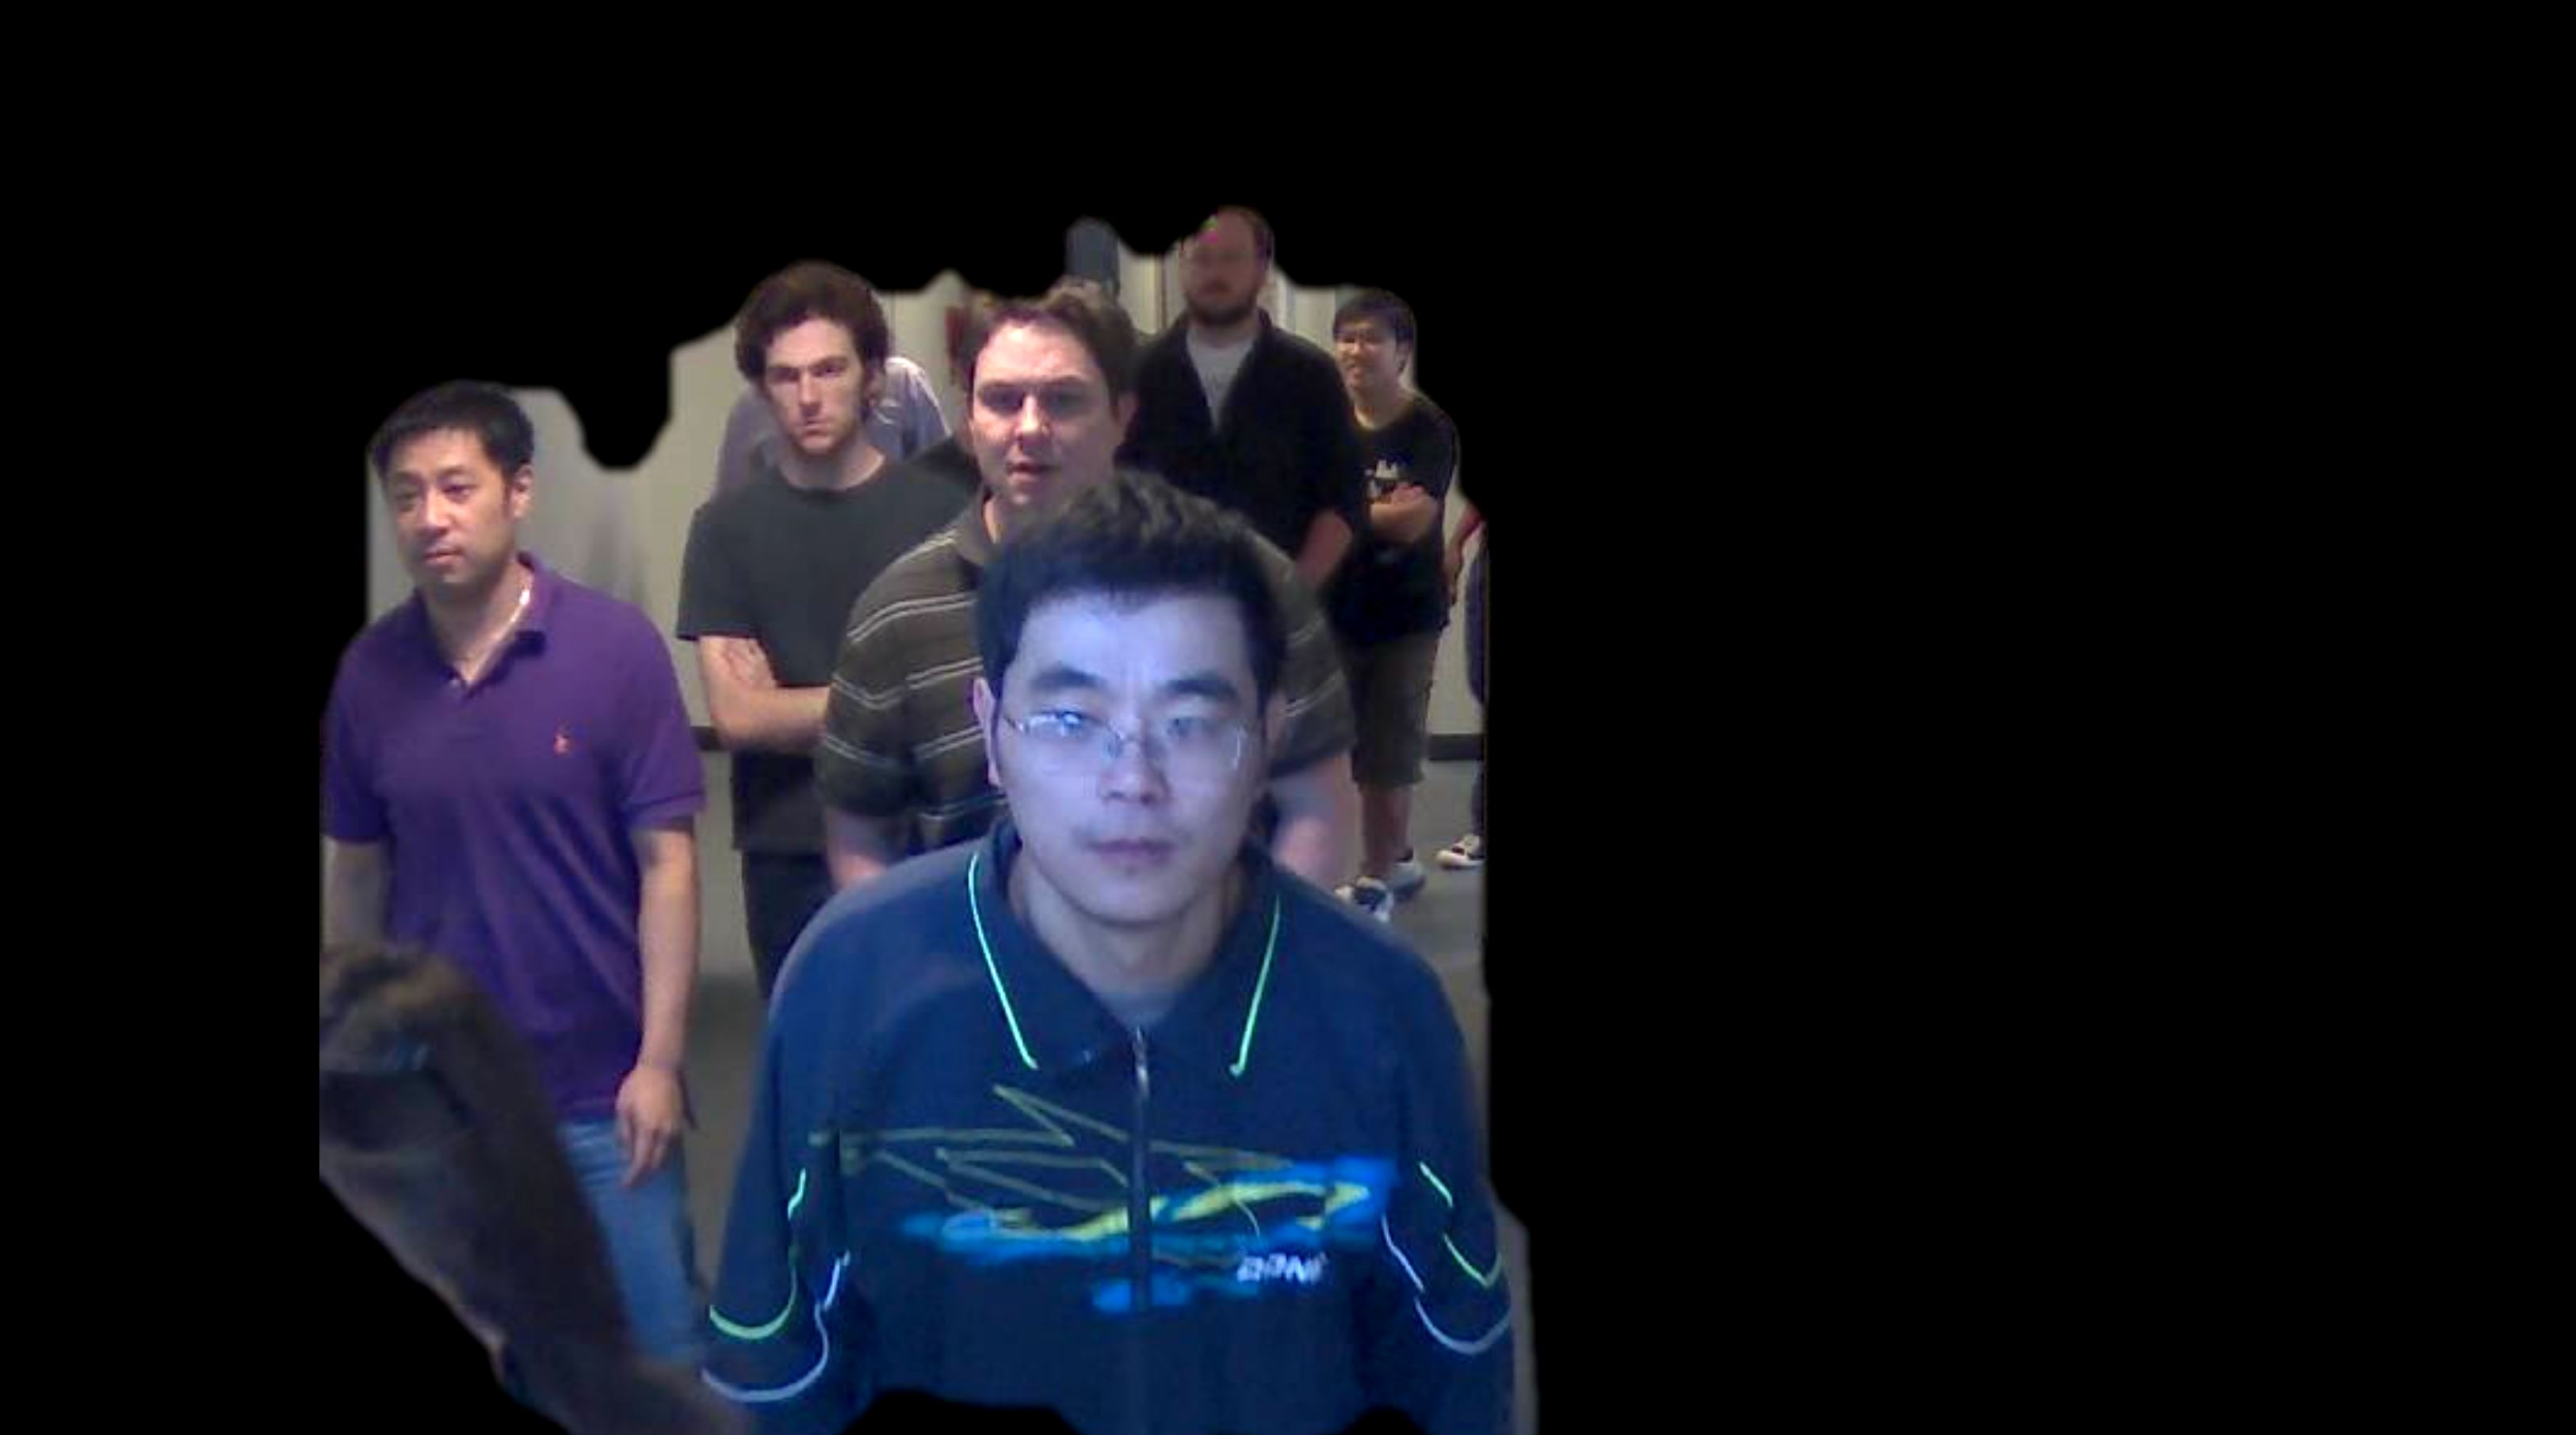
\includegraphics[width=12cm]{P2L_S5}
	\caption{rendered image from P2LS5}
	\label{fig:rendered image from P2LS5}
\end{figure}

\begin{figure}[h]
	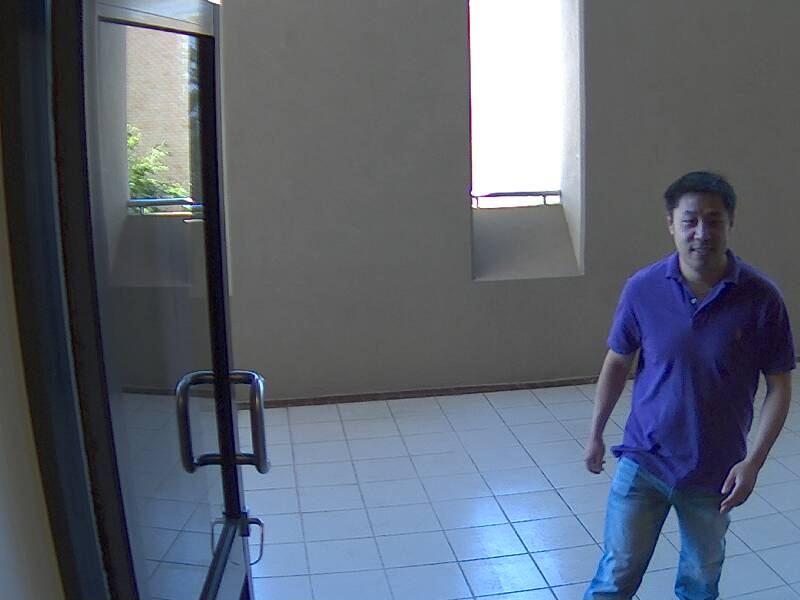
\includegraphics[width=12cm]{P2E_S2_ori}
	\caption{original image from P2LS5}
	\label{fig:original image from P2LS5}
\end{figure}

\begin{figure}[h]
	
\includegraphics[width=12cm]{P2E_S2}
	\caption{rendered image from P2ES2}
	\label{fig:rendered image from P2ES2}
\end{figure}

\begin{figure}[h]
	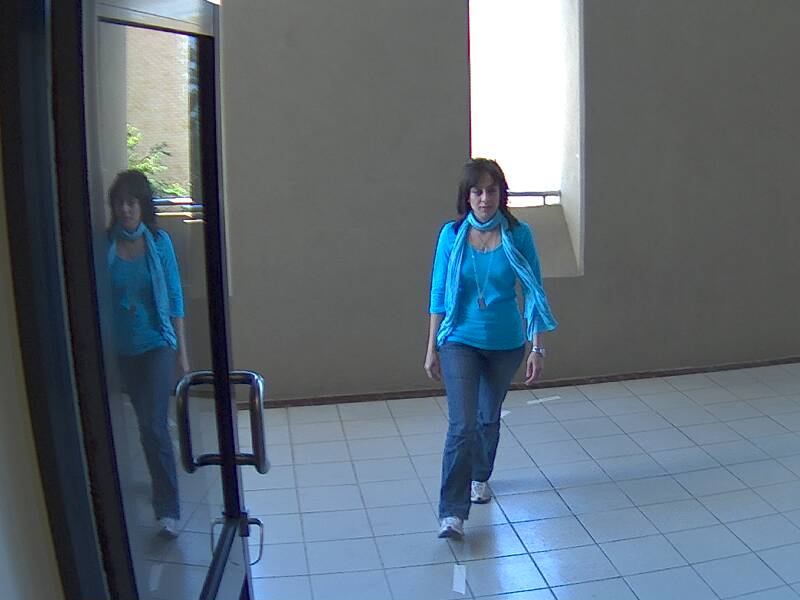
\includegraphics[width=12cm]{P2E_S4_ori}
	\caption{original image from P2ES4}
	\label{fig:original image from P2ES4}
\end{figure}

\begin{figure}[h]
	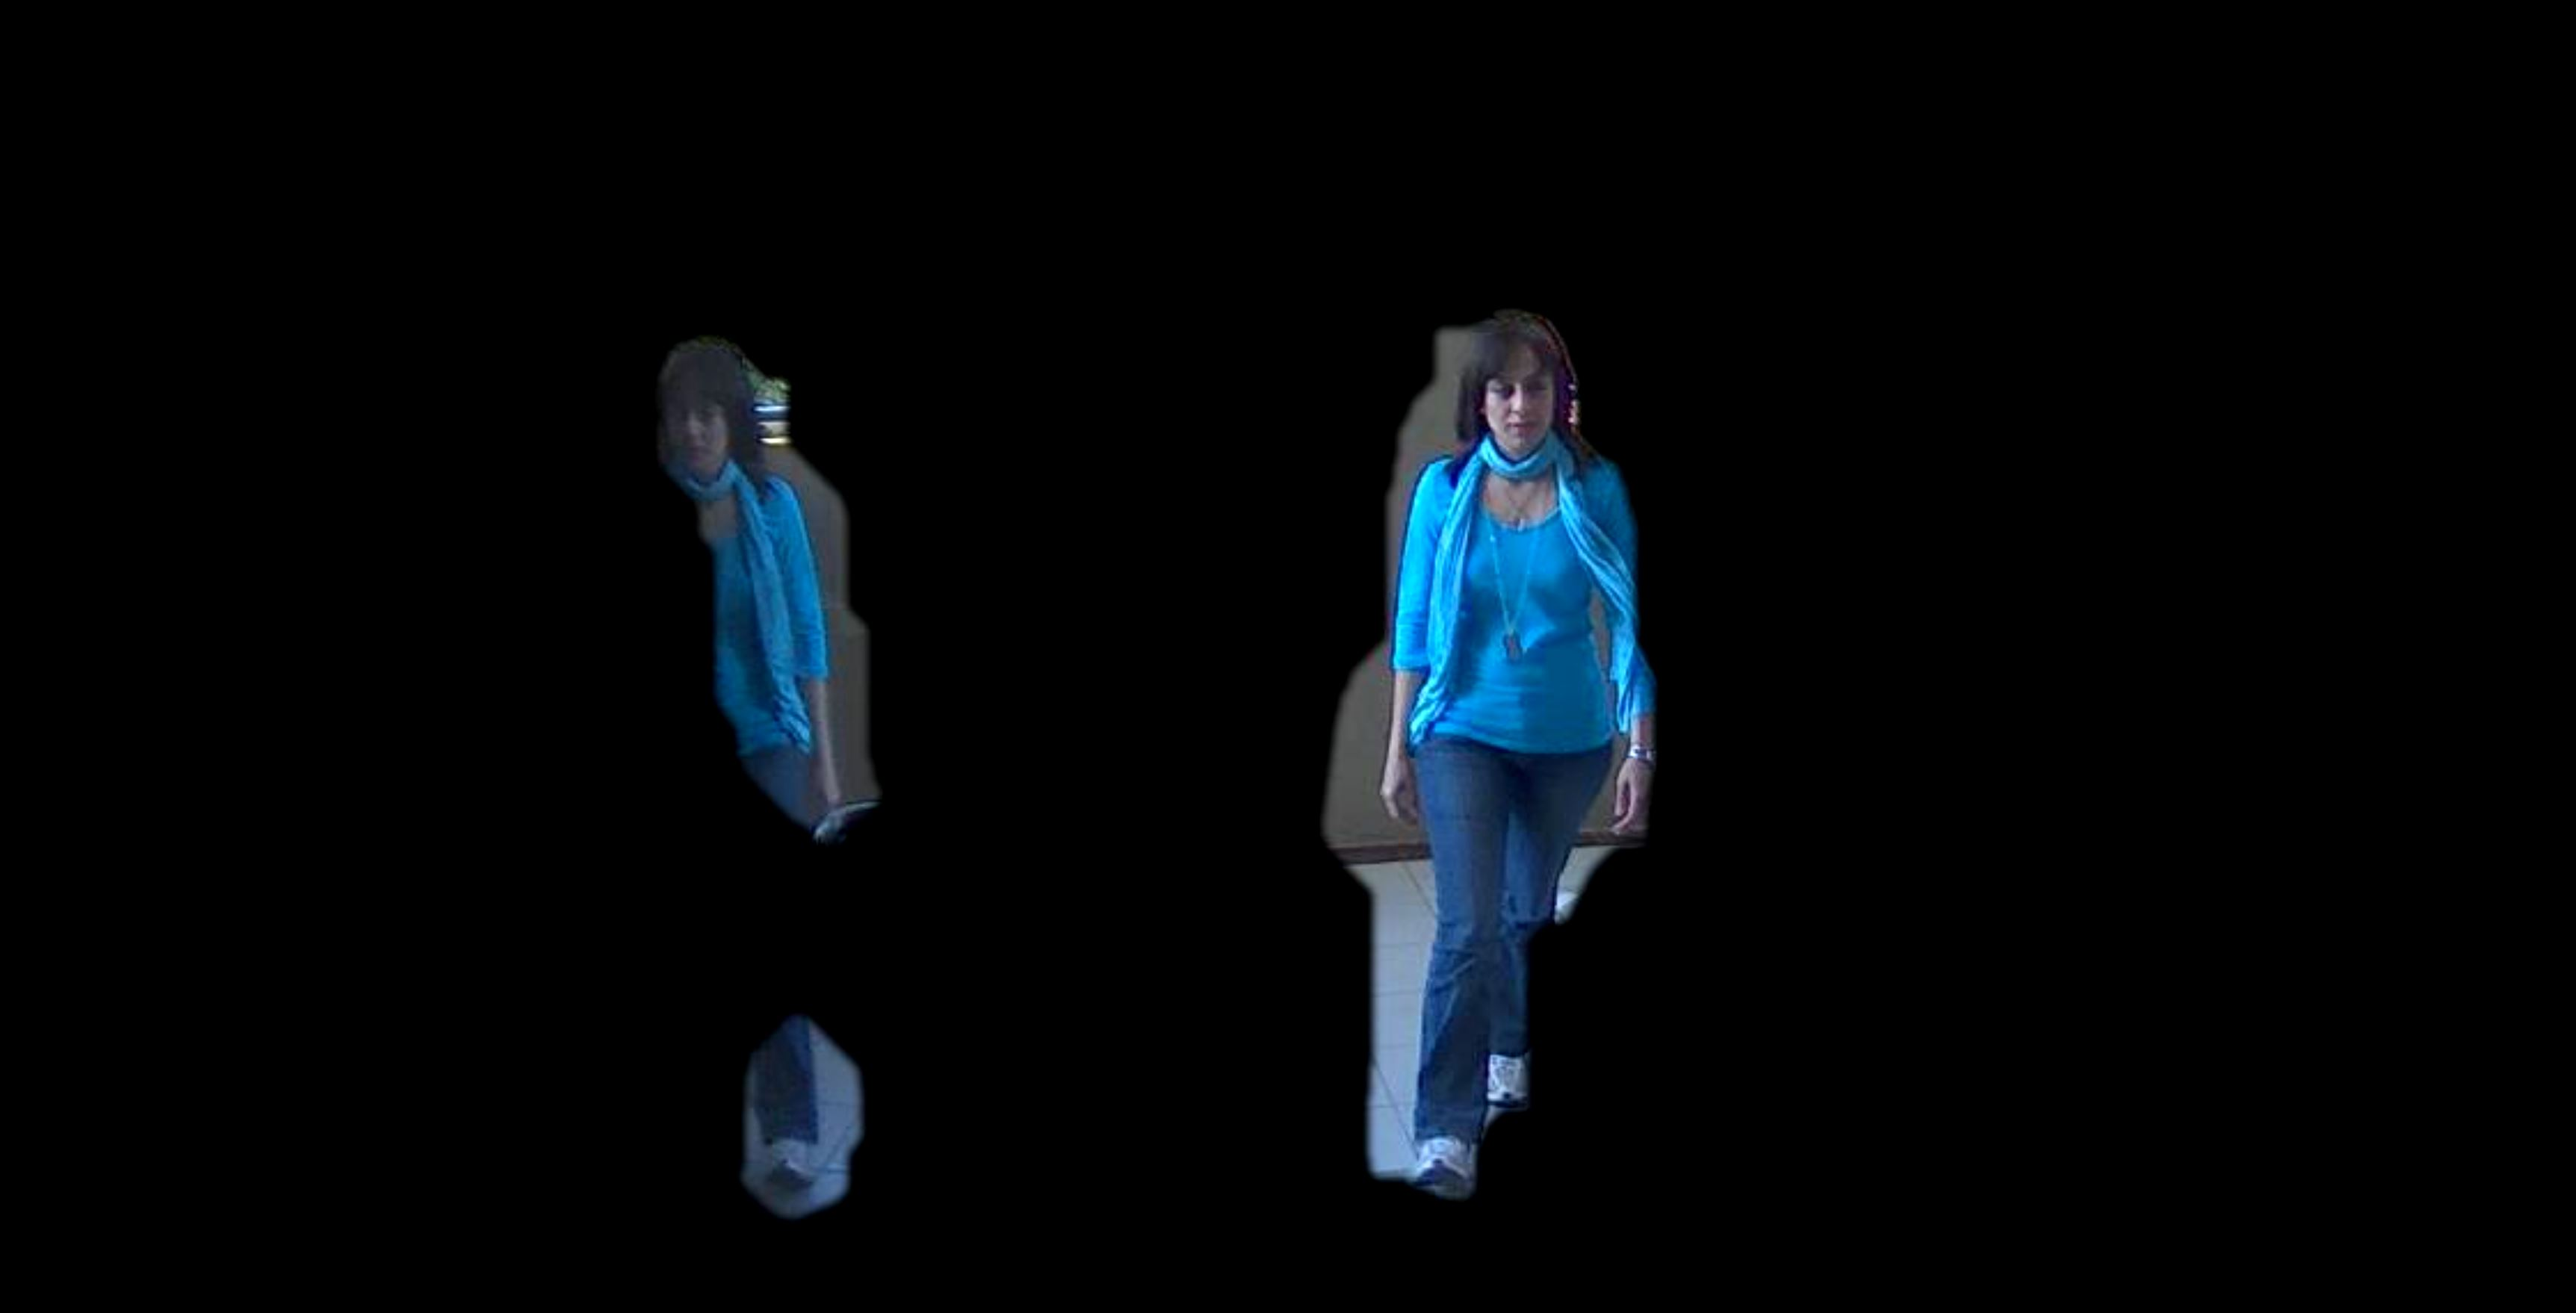
\includegraphics[width=12cm]{P2E_S4}
	\caption{rendered image from P2ES4}
	\label{fig:rendered image from P2ES4}
\end{figure}

\begin{figure}[h]
	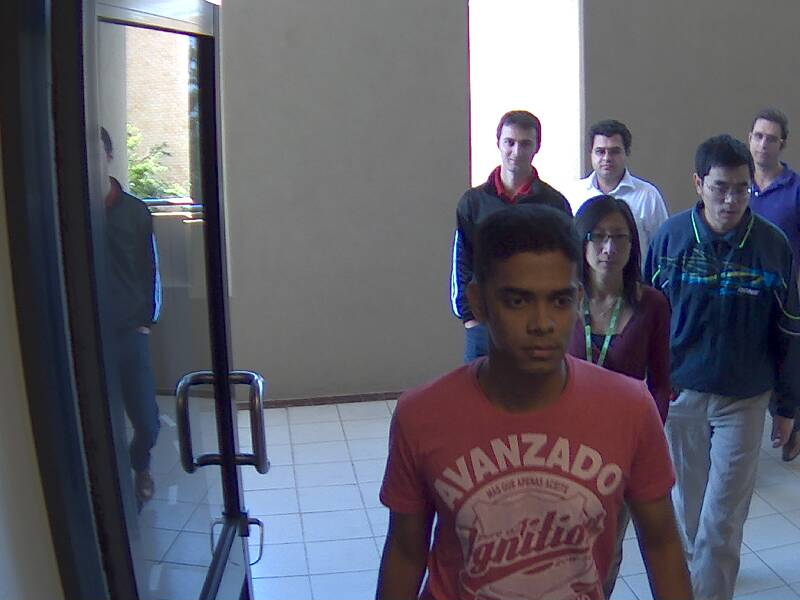
\includegraphics[width=12cm]{P2E_S5_ori}
	\caption{original image from P2ES5}
	\label{fig:original image from P2ES5}
\end{figure}

\begin{figure}[h]
	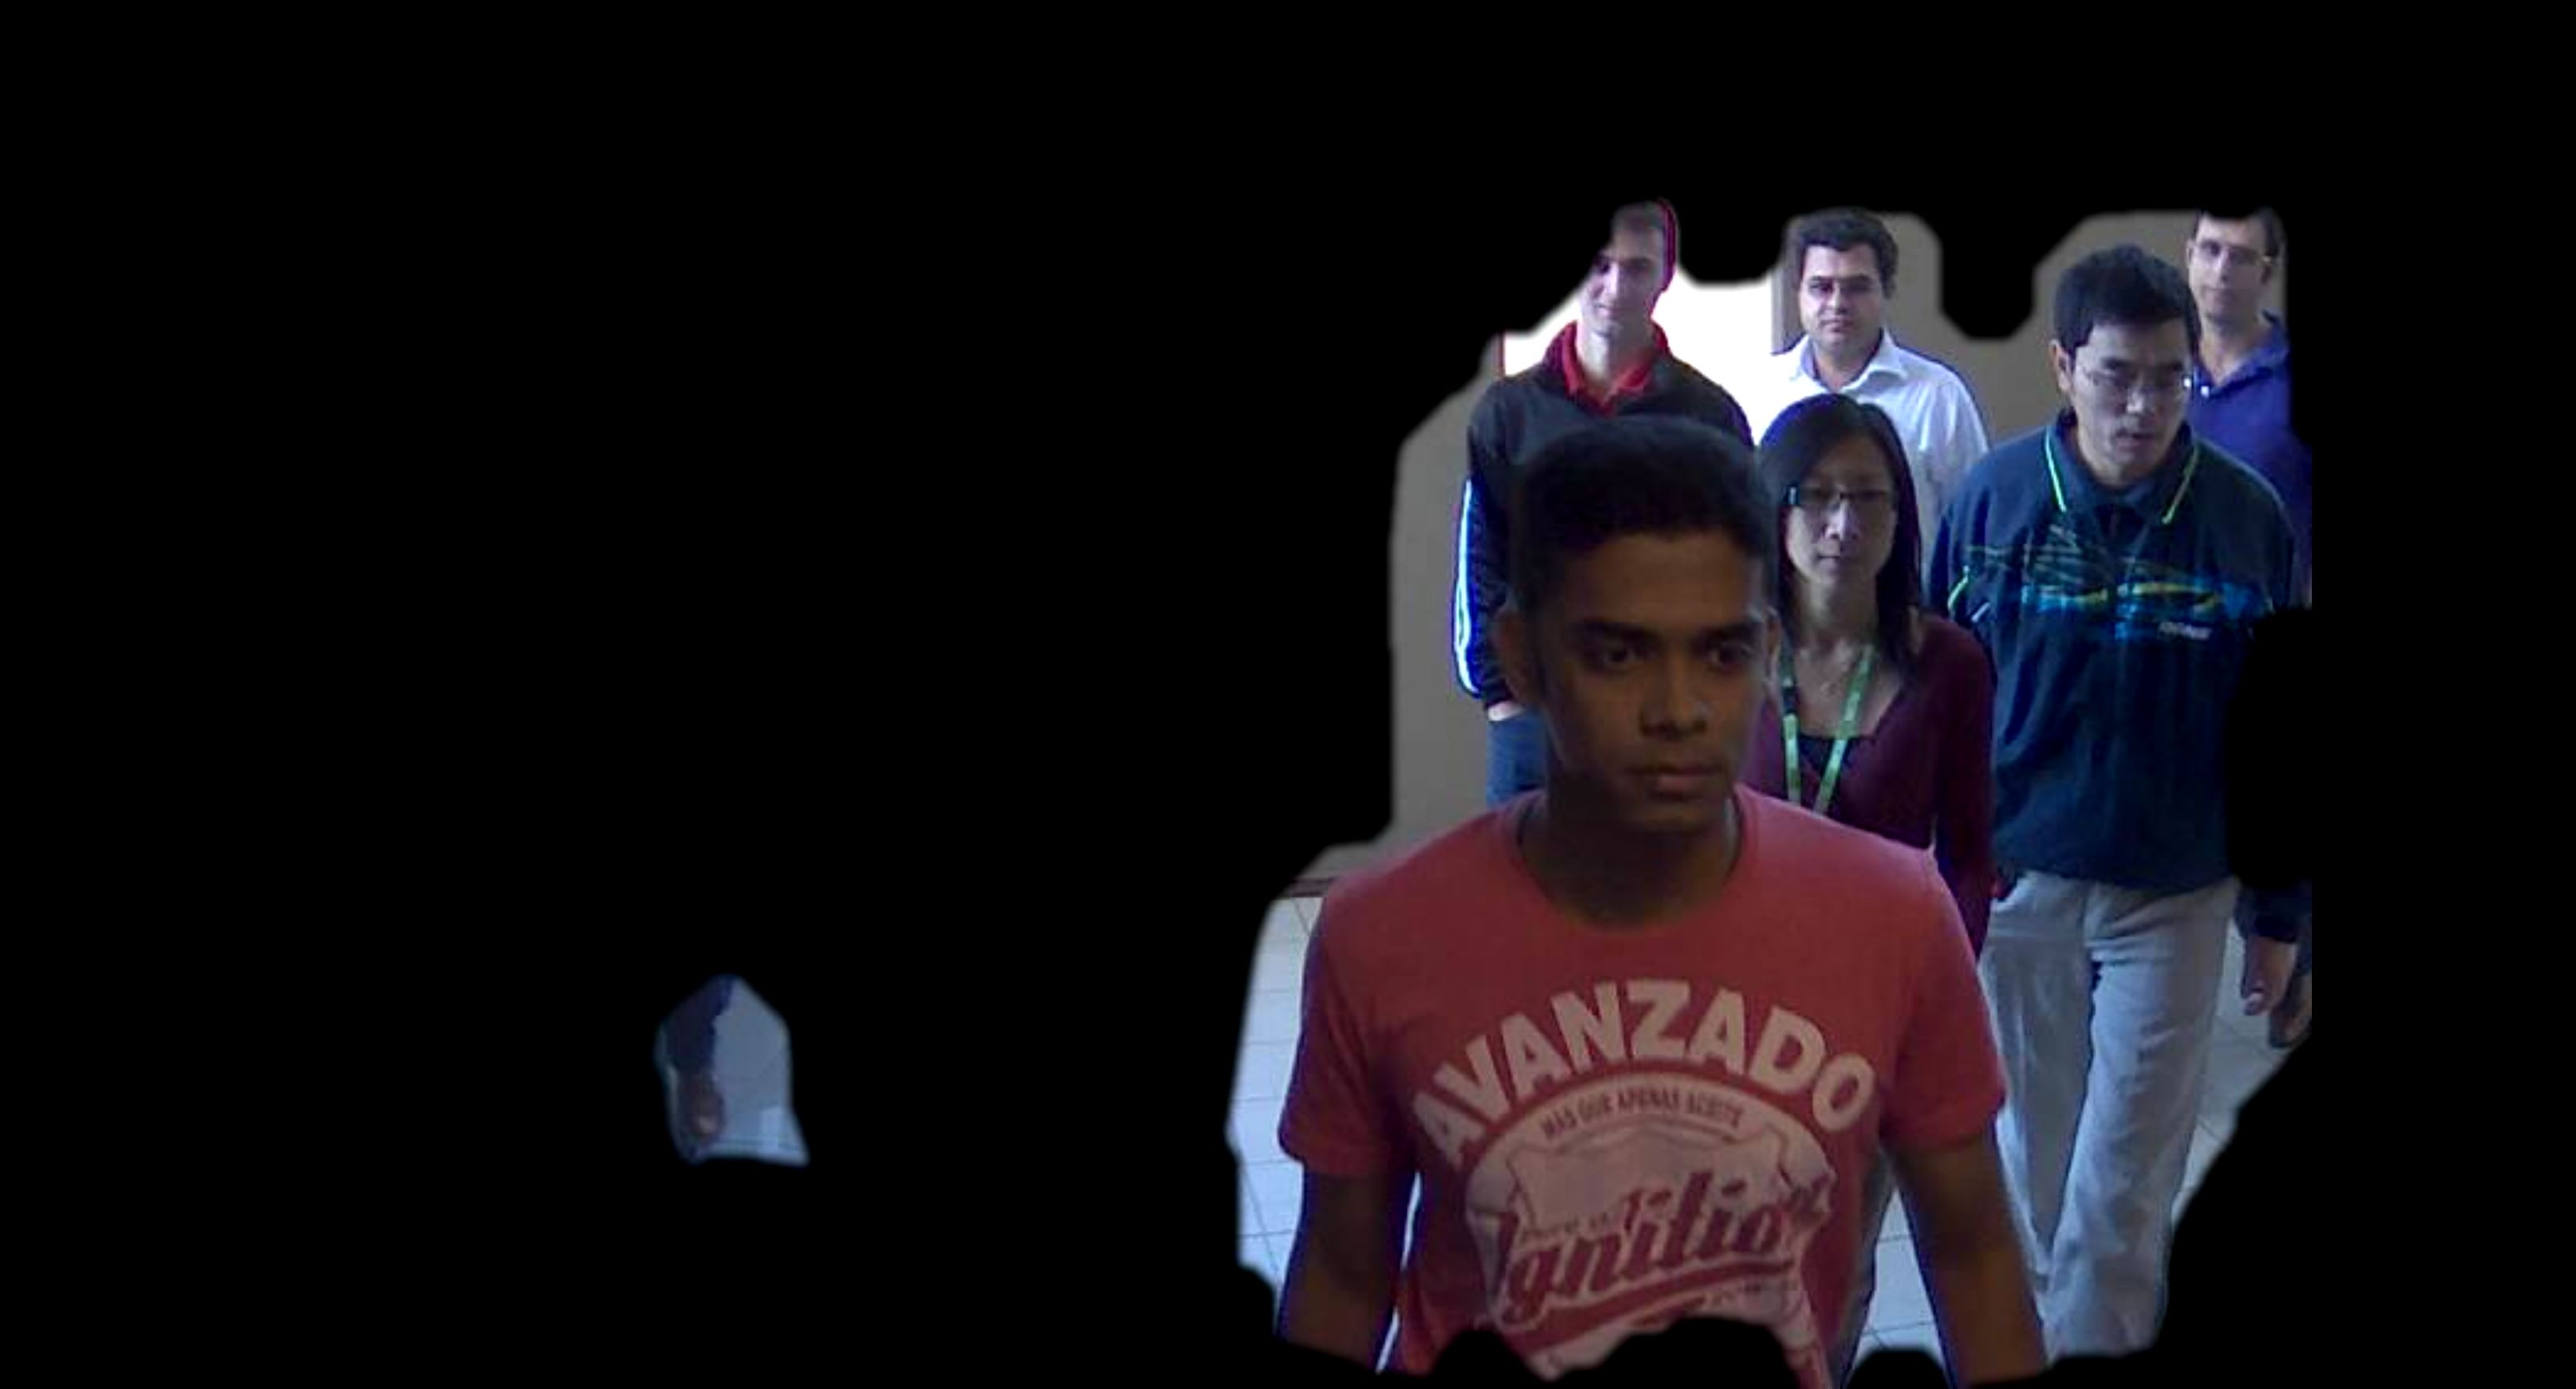
\includegraphics[width=12cm]{P2E_S5}
	\caption{rendered image from P2ES5}
	\label{fig:rendered image from P2ES5}
\end{figure}

The segmentation using Gaussian Mixture Models has proven to be successful. As we can see in the following illustrations, moving individuals or objects are recognised as being a part of the foreground. The model is also robust to changes in lighting, however, it has flaws that can be improved on. 


First, as seen in the figure ~\ref{fig:original image from P2ES4}, shadows and reflections of moving objects are considered as being part of the foreground. \\

Then, due to the model only considering the changes in the variance of a pixel, moving objects with the same colour as the background will not be recognised. The torso of an individual wearing a strapped shirt matching the gray floor will be cut by the mask. This can be seen in the figure ~\ref{fig:original image from P1LS3}

Furthermore, as the figure ~\ref{fig:original image from P2LS5} shows, the model is robust when working with a large crowd. Everyone in the foreground will be efficiently distinguished.
Finally, slow moving objects will be ignored as well if the change in the variance does not exceed the threshold. 


\subsection{Video}

\section{Conclusion \& Outlook} 
In conclusion, we have reached our goal and created a functioning foreground detection and segmentation algorithm. Even though our project is successfull, it can still be refined. First of all, Slow moving objects should also be recognised as being part of the foreground. Then, the robustness of the algorithm against shadows and reflections should also be improved. Finally, a new concept should be developed in order to differentiate between background and foreground of the similar colour.  
\end{document}

\subsection{Laufzeit Benchmark}
Zur Evaluierung der Ausführungsdauer unseres Algorithmus haben wir verschiedene virtuelle Ansichten auf unterschiedlichen Systemen berechnet und dabei die Laufzeiten gestoppt. Um zuverlässigere Ergebnisse zu bekommen, haben wir die selbe Berechnung mehrmals ausgeführt und anschließend den Mittelwert und die Standardabweichung der Laufzeit berechnet. So haben wir die virtuellen Ansichten für $p \in [0.2, 0.45, 0.7, 1]$ jeweils 5 mal für beide Bildpaare berechnet, um schließlich die Laufzeiten von insgesamt 40 Durchläufen der Funktion $free\_viewpoint$ zu erhalten. Dabei ergaben sich die in Tabelle \ref{tab:evaluierung_laufzeiten} dargestellten Ergebnisse.

\begin{table}[htbp]
	\begin{center}
		\begin{tabular}{c|c|c|c}
			& System 1 & System 2 & System 3 \\ \hline
			\begin{tabular}[c]{@{}c@{}}Laufzeit\\ mean (std) \end{tabular} & 131,4s (77,4s) & 149,8s (95,1s) & 241,5s (154,6s) \\ \hline
			CPU & \begin{tabular}[c]{@{}c@{}}Intel Core i7 - 7700K  \\ 4 x 4,4 GHz \end{tabular} & \begin{tabular}[c]{@{}c@{}}Intel Core i5 - 4590\\ 4 x 3,3 GHz \end{tabular} & \begin{tabular}[c]{@{}c@{}}Intel Core i5\\ 2 x 2,6 GHz \end{tabular} \\ \hline
			RAM & \begin{tabular}[c]{@{}c@{}}16 GB\\ 2133 MHz \\ DDR4 \end{tabular} & \begin{tabular}[c]{@{}c@{}}8 GB\\ 2133 MHz \\ DDR3  \end{tabular} & \begin{tabular}[c]{@{}c@{}}8 GB\\ 1600 MHz \\ DDR3  \end{tabular} \\ \hline
			OS & \begin{tabular}[c]{@{}c@{}}Windows 10 \\ 1803 17134 \end{tabular} & \begin{tabular}[c]{@{}c@{}}Windows 10 \\ 1803 17134  \end{tabular} & \begin{tabular}[c]{@{}c@{}}macOS High Sierra \\ Version 10.13.6  \end{tabular}
		\end{tabular}
		\caption{Evaluierung der Ausführungszeiten auf drei verschiedenen Systemen}
	\end{center}
	\label{tab:evaluierung_laufzeiten}
\end{table}

Eine eigene Evaluierung der Laufzeit kann mit Hilfe des Skriptes $benchmark.m$ im Ordner \textit{/src} des Projektes durchgeführt werden. Die Ergebnisse des Benchmarks werden automatisch im Ordner \textit{/out} gespeichert.
